\chapter{Wstępy}

\section{02.10.2024}{Grafy Cayleya}

\subsection{Metryka słów}

\begin{definition}{metryka słów}{}
  Niech $G$ będzie grupą, a $S$ dowolnym układem jej generatorów. Wówczas dla dowolnych $g_1,g_2\in G$ \buff{odległość między nimi w metryce słów} definiujemy jako
$$ds(g_1, g_2)=\min\{n\;:\;g_2=g_1s_1,...,s_n,\;s_i\in S\cup S^{-1}\},$$
gdzie $S^{-1}=\{g^{-1}\;:\;g\in S\}$.
\end{definition}

Metryka słów jest 
\begin{enumerate}
  \item skończona
  \item symetryczna (z definicji generatorów)
  \item \hl{lewo-niezmiennicza}, czyli $(\forall\;\gamma\in G)\;ds(\gamma g_1,\gamma g_2)=ds(g_1, g_2)$
\end{enumerate}
Ostatnia własność oznacza, że $G$ działa na sobie jako na przestrzeni metrycznej przez izometrie.

Gromov chce patrzeć na dyskretne przestrzenie metryczne, jakimi są grupy z metryką słów, jako na przestrzenie ciągłe (z dużej odległości).

\subsection{Graf Cayleya}

\begin{definition}{graf Cayleya}{}
Niech $G$ będzie grupą, a $S$ zbiorem jej generatorów. $C(G, S)$ to graf Cayleya o wierzchołkach będących elementami $G$ i skierowanych krawędziach etykietowanych generatorami:
\begin{center}
  \begin{tikzcd}
    g\arrow["s", r] & gs
  \end{tikzcd}
\end{center}
gdzie $g\in G$ i $s\in S$.
\end{definition}

\begin{example}[m]
\item Dla $G=\Z^2$ oraz $S=\{{\color{red}\overbrace{(1, 0)}^s}, {\color{blue}\overbrace{(0, 1)}^t}\}$ graf Cayleya to nieskończona "kratka"
  \bigskip

  \begin{center}
    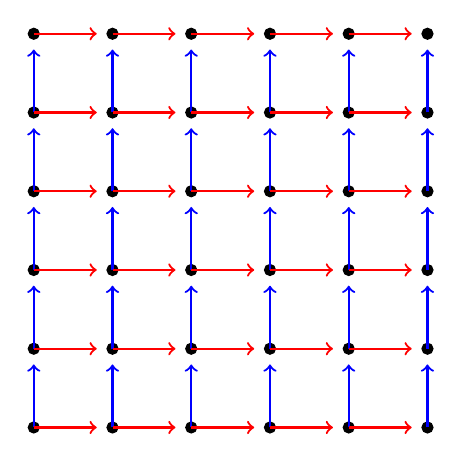
\begin{tikzpicture}
      \foreach \x in{0,...,5} { 
        \foreach \y in{0,...,5} {
          \filldraw (\x, \y) circle (2pt);
        }
      }

      \foreach \x in {0,...,5} {
        \foreach \y in {0,..., 4} {
          \draw[->, blue, thick] (\x, \y) -- (\x, \y+.8);
        }
      }
      \foreach \x in {0,...,4} {
        \foreach \y in {0,..., 5} {
          \draw[->, red, thick] (\x, \y) -- (\x+.8, \y);
        }
      }
    \end{tikzpicture}
  \end{center}
\item Dla grupy cyklicznej rzędu $p$ z generatorem $\color{red}s$ graf Cayleya to $p$-kąt
  \begin{center}
    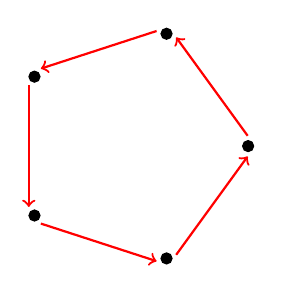
\begin{tikzpicture}
      \foreach \i in {0,..., 4} {
        \filldraw ( 360 /5 * \i :1.5) circle (2pt);
        \draw[->, red, thick] (360/5*\i + 5:1.5) -- (360/5*\i + 360/5 - 5:1.5);
      }
    \end{tikzpicture}
  \end{center}
\item {\color{red}\Large TO DO} parkietarz kwadratami
\end{example}

Innym wariantem grafu Cayleya niż zdefiniowany wcześniej jest graf w którym wierzchołki są elementami grupy $V=G$, ale krawędzie są niezorientowane: $E=\{\{g_1, g_2\}\;:\;ds(g_1,g_2)=1\}$. W przykładzie z parkietarzem zamiast podwójnych krawędzi w obie strony będzie on miał pojedyńczą, nieskierowaną krawędź

Każdy graf Cayleya jest \buff{spójny}, bo jego krawędzie to mnożenie przez generatory. Dodatkowo, grupa $G$ działa na nim przez \hl{automorfizmy zachowując krawędzie oraz ich etykiety}. To znaczy, że krawędż z wierzchołkami 
\begin{center}\begin{tikzcd}g\arrow[r, "s"]&gs\end{tikzcd}\end{center} 
pod działaniem elementu $\gamma \in G$ staje się 
\begin{center}\begin{tikzcd}\gamma g\arrow[r, "s"] & \gamma gs.\end{tikzcd}\end{center}

Jeśli każdą krawędź w grafie Cayleya potraktujemy jako odcinek długości $1$, to możemy na nim zdefiniować metrykę która jako odległość dwóch punktów przyjmuje długość najkrótszej ścieżki między nimi. Ta metryka na wierzchołkach pokrywa się z \buff{metryką słów} na grupie $G$ o generatorach $S$, której graf rozpatrujemy. Przy takiej metryce działanie grupy \hl{$G$ jest więc działaniem nie tylko przez automorfizmy, ale przez izometrie} (lewa-niezmienniczość).


Dla surjekcji $\pi:F_S\to G$, gdzie $G=\langle S\;|\; R\rangle=F_S/N$ możemy mieć dwie tak samo zorientowane strzałki między dwoma wierzchołkami (gdy np. $g_1\pi(s_1)=g_1\pi(s_2)=g_2$
\begin{center}
  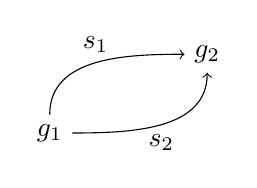
\begin{tikzpicture}
    \node (g1) at (0, 0) {$g_1$};
    \node (g2) at (2, 1) {$g_2$};
    \draw[->] (g1) to [out=90, in=180] node[midway, above] {$s_1$} (g2);
    \draw[->] (g1) to [out=0, in=-90] node[midway, below] {$s_2$} (g2);
  \end{tikzpicture}
\end{center}

% Graf Cayleya grupy wolnej to nieskończone drzewo stopnia równego ilości $2\cdot$ ilość generatorów. 

\begin{definition}{suma drzewiasta}{}
  Mając dwie grupy $(G_1, S_1)$ i $(G_2, S_2)$ graf Cayleya ich sumy wolnej, czyli graf $(G_1\star G_2, S_1\cup S_2)$ to graf pierwszej grupy, który w każdym wierzchołku ma kopię grafu drugiej grupy, która w każdym wierzchołku ma kopię pierwszej grupy...

  \begin{center}
    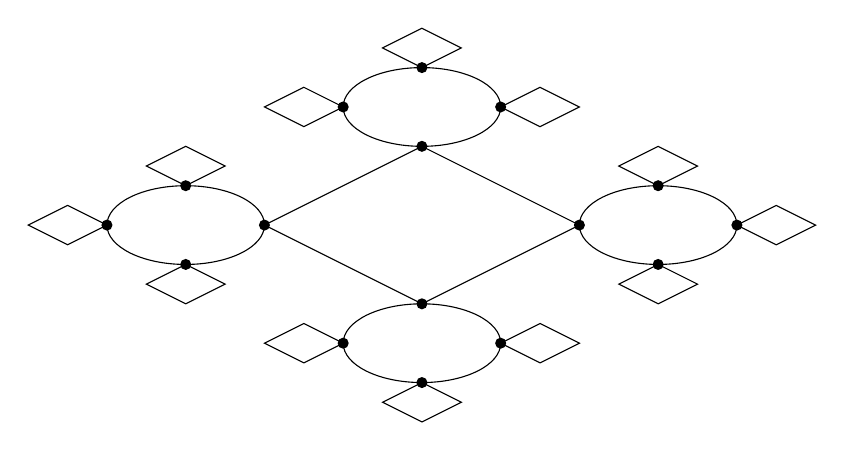
\begin{tikzpicture}
      \fill (-2, 0) circle (2pt);
      \fill (2, 0) circle (2pt);
      \fill(0,1)circle(2pt);
      \fill(0,-1)circle(2pt);
      \draw (2,0)--(0,1)--(-2,0)--(0,-1)--(2,0);

      \draw (0, 1.5) ellipse (1 and 0.5);
      \fill (0,2) circle (2pt);
      \fill(1, 1.5) circle (2pt);
      \fill(-1, 1.5) circle (2pt);
      
      \draw (0, -1.5) ellipse (1 and 0.5);
      \fill (0,-2) circle (2pt);
      \fill(1, -1.5) circle (2pt);
      \fill(-1, -1.5) circle (2pt);
      
      \draw (3, 0) ellipse (1 and 0.5);
      \fill (4,0) circle (2pt);
      \fill(3, .5) circle (2pt);
      \fill(3, -.5) circle (2pt);
      
      \draw (-3, 0) ellipse (1 and 0.5);
      \fill (-4,0) circle (2pt);
      \fill(-3, .5) circle (2pt);
      \fill(-3, -.5) circle (2pt);

      \draw (0, 2)--(.5, 2.25)--(0,2.5)--(-.5, 2.25)--cycle;
      \draw (1, 1.5)--(1.5, 1.25)--(2,1.5)--(1.5, 1.75)--cycle;
      \draw (-1, 1.5)--(-1.5, 1.25)--(-2,1.5)--(-1.5, 1.75)--cycle;

      \draw (1, -1.5)--(1.5, -1.25)--(2,-1.5)--(1.5, -1.75)--cycle;
      \draw (-1, -1.5)--(-1.5, -1.25)--(-2,-1.5)--(-1.5, -1.75)--cycle;
      \draw (0, -2)--(.5, -2.25)--(0,-2.5)--(-.5, -2.25)--cycle;

      \draw (3, .5)--(3.5, .75)--(3, 1)--(2.5, .75)--cycle;
      \draw (3, -.5)--(3.5, -.75)--(3, -1)--(2.5, -.75)--cycle;
      \draw (4, 0)--(4.5, -.25)--(5, 0)--(4.5, .25)--cycle;

      \draw (-3, .5)--(-3.5, .75)--(-3, 1)--(-2.5, .75)--cycle;
      \draw (-3, -.5)--(-3.5, -.75)--(-3, -1)--(-2.5, -.75)--cycle;
      \draw (-4, 0)--(-4.5, -.25)--(-5, 0)--(-4.5, .25)--cycle;
    \end{tikzpicture}
  \end{center}
\end{definition}

\subsection{Quasi-izometrie}

\begin{definition}{quasi-izometria}{}
  Dla dwóch przestrzeni metrycznych $(X_i, d_i)$, $i=1,2$, mówimy, że przekształcenie $f:X_1\to X_2$ (niekoniecznie ciągłe) jest \buff{quasi-izometryczne zanurzenie}, gdy istnieje $C\geq 1$ oraz $L\geq 0$ takie, że $\forall\;x,y\in X_1$ zachodzi
  $$\frac{1}{C}d_1(x,y)-L\leq d_2(f(x),f(y))\leq C\cdot d_1(x,y)+L.$$

  Ponadto, jeśli istnieje $D\geq 0$ takie, że $f(X_1)$ jest $D$-gęsty ($D$-siecią) w $X_2$, tzn. 
  $$(\forall\;y\in X_2)(\exists\;x\in X_1)\;d_2(y, f(x))\leq D$$
  to wtedy $f$ jest \buff{quasi-izometrią}.
\end{definition}

Zwykle przyjmujemy $L=D$ (większe z dwóch) i mówimy o tzw. \hl{(C, L)-quasi-izometrii}.

\begin{fact}{własności q.i.}{}
  \begin{enumerate}
    \item złożenie q.i. jest q.i
    \item dla dowolnej q.i. $f:X_1\to X_2$ istnieje $g:X_2\to X_1$ takie, że istnieje $D\geq 0$ takie, że
      $$(\forall\;x_2\in X_2)\;d_2(f\circ g(x_2), x_2)\leq D$$
      $$(\forall\;x_1\in X_1)\;d_1(g\circ f(x_1), x_1)\leq D$$
      to wówczas $g$ też jest q.i.
  \end{enumerate}
\end{fact}

\begin{definition}{quasi-izometryczne rozmaitości}{}
  Mówimy, że $(X_1, d_1)$ jest quasi-izometryczna z $(X_2, d_2)$ jeśli istnieje q.i. $f:X_1\to X_2$. Jest to relacja równoważności.
\end{definition}

\begin{example}[m]
  \item $(X, d)$ jest q.i. z punktem $\iff$ $X$ jest ograniczone.
  \item $X$ jest q.i. z dowolną swoją $D$-siecią $Y\subseteq X$ przez inkluzję.
  \item Dla dowolnego $B$ ograniczonego $X\times B\cong X$ są q.i.
  \item Dowolne dwa drzewa regularne $T_k$ stopnia $k\geq 3$ są ze sobą q.i.
  \item Graf Farey'a, nieskończony konstruowany jak niżej, z metryką kombinatoryczną (każda krawędź ma długość 1) jest q.i. z drzewem przeliczalnego stopnia $T_\omega=T_{\aleph_0}$.
    \begin{center}
      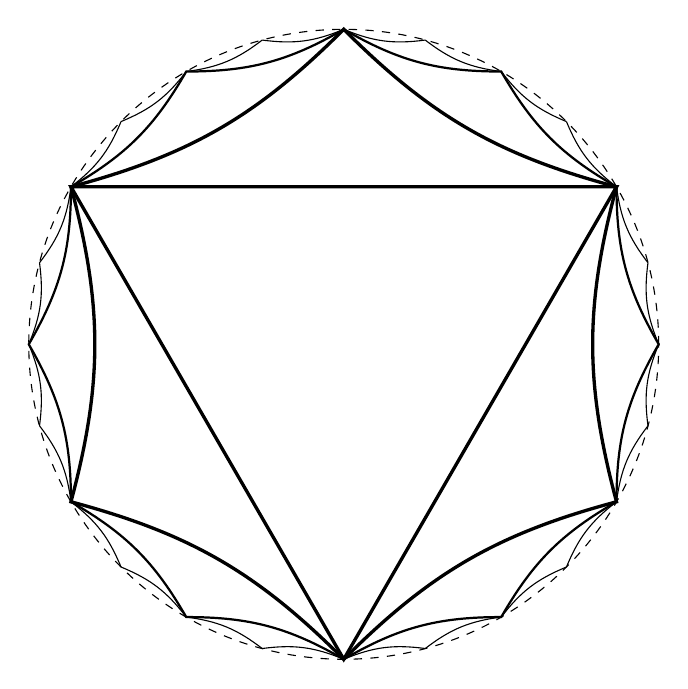
\begin{tikzpicture}
        \draw[dashed] (0,0) circle (4);
        \draw[very thick] ({4*cos(30)}, {4*sin(30)})--({4*cos(150)}, {4*sin(150)})--(0, -4)--cycle;
        \draw[very thick] ({4*cos(30)}, {4*sin(30)}) to[bend left=15] (0, 4) to[bend left=15] ({4*cos(150)}, {4*sin(150)})to[bend left=15]({4*cos(210)}, {4*sin(210)})to[bend left=15](0, -4)to[bend left=15]({4*cos(-30)}, {4*sin(-30)}) to[bend left=15]cycle;
        \draw[thick] ({4*cos(30)}, {4*sin(30)}) to[bend left=15] ({4*cos(60)}, {4*sin(60)}) to[bend left=15] (0, 4) to[bend left=15]({4*cos(120)},{4*sin(120)})to[bend left=15] ({4*cos(150)}, {4*sin(150)}) to[bend left=15]({4*cos(180)},{4*sin(180)})to[bend left=15]({4*cos(210)}, {4*sin(210)})to[bend left=15]({4*cos(240)}, {4*sin(240)})to[bend left=15](0, -4)to[bend left=15]({4*cos(-60)}, {4*sin(-60)})to[bend left=15]({4*cos(-30)}, {4*sin(-30)})to[bend left=15](4,0)to[bend left=15]cycle;

        \foreach \i in {0, 15, 30, ..., 345} {
          \draw ({4*cos(\i)}, {4*sin(\i)}) to[bend left=15] ({4*cos(\i+15)}, {4*sin(\i+15)});
        }
      \end{tikzpicture}
    \end{center}
\end{example}

\begin{fact}{}{}
  Niech $G$ będzie grupą skończenie generowalną i niech $S_1$, $S_2$ jej skończonymi zbiorami generatorów. Wówczas odwzorowanie tej grupy jako dwóch przestrzeni metrycznych $(G, S_1)\to (G, S_2)$ gdzie zmieniamy metrykę słów jest q.i.
\end{fact}

\begin{conc}{}{}
  Skończenie generowana grupa $G$ determinuje jednoznacznie klasę quasi-izometrii. Innymi słowy, skończenie generowana grupa jest \hl{jednoznacznym obiektem quasi-metrycznym}.
\end{conc}

